% Clase de documento
\documentclass[letterpaper,12pt,oneside]{book}
% Paquetes
\usepackage[utf8]{inputenc}                                           % Codificación de caracteres
\usepackage[T1]{fontenc}                                              % Codificación de salida
\usepackage[spanish,es-nodecimaldot,es-tabla]{babel}                  % Idioma español
\usepackage{graphicx}                                                 % Para insertar imágenes
\usepackage[top=1in, left=0.9in, right=1.25in, bottom=1in]{geometry}  % Márgenes
\usepackage{tikz}                                                     % Para crear gráficos
\usepackage{tocloft}                                                  % Para personalizar la tabla de contenido
\usepackage{setspace}                                                 % Para el interlineado
\usepackage[backend=biber,style=numeric]{biblatex}                    % Para la bibliografía
\usepackage{csquotes}                                                 % Para citas bibliográficas
\usepackage{amsmath}                                                 % Para ecuaciones matemáticas
\graphicspath{{./Imágenes/}}                                          % Ruta de las imágenes

% Archivo de bibliografía
\addbibresource{references.bib}

\begin{document}

    
\begin{titlepage}
    \thispagestyle{empty}
    \begin{minipage}[c][0.17\textheight][c]{0.23\textwidth}
        \begin{center}
            
\includegraphics[width=3.5cm, height=3.5cm]{Escudo-UNAM.pdf}
        \end{center}
    \end{minipage}
    \begin{minipage}[c][0.195\textheight][t]{0.725\textwidth}
        \begin{center}
            \vspace{0.3cm}
            \textsc{\large Universidad Nacional Aut\'onoma de M\'exico}\\[0.5cm]
            \vspace{0.3cm}
            \hrule height2.5pt
            \vspace{.2cm}
            \hrule height1pt
            \vspace{.8cm}
            \textsc{Facultad de Química}\\[0.5cm] %
        \end{center}
    \end{minipage}

    \begin{minipage}[c][0.81\textheight][t]{0.20\textwidth}
        \vspace*{5mm}
        \begin{center}
            \hskip2.0mm
            \vrule width1pt height13cm 
            \vspace{5mm}
            \hskip2pt
            \vrule width2.5pt height13cm
            \hskip2mm
            \vrule width1pt height13cm \\
            \vspace{5mm}
            
\includegraphics[height=3.2cm]{logofq.jpeg}
        \end{center}
    \end{minipage}
    \begin{minipage}[c][0.81\textheight][t]{0.75\textwidth}
        \begin{center}
            \vspace{1cm}

            {\large\scshape Estudio de la solvatación del ion Cu\textsuperscript{2+} en agua y metanol mediante dinámica molecular con DFT/M06-2X}\\[.2in]

            \vspace{2cm}            

            \textsc{\LARGE T\hspace{1.5cm}E\hspace{1.5cm}S\hspace{1.5cm}I\hspace{1.5cm}S}\\[0.5cm]
            \textsc{\large que para obtener el t\'itulo de:}\\[0.5cm]
            \textsc{\large Ingeniero Químico}\\[0.5cm]
            \textsc{\large presenta:}\\[0.5cm]
            \textsc{\large {Jorge Angel Rosas Martínez}}\\[2cm]          

            \vspace{0.5cm}

            {\large\scshape Tutores:\\[0.3cm] {Dr. César Iván León Pimentel}}\\[.2in]

            \vspace{0.5cm}

            \large{Ciudad Universitaria, CDMX}{ }{2025}
        \end{center}
    \end{minipage}
\end{titlepage}


    \frontmatter % Páginas preliminares

        \chapter*{Dedicatoria}
\begin{flushright}
  \emph{Dedicatoria ...} \\
  Hola, soy la dedicatoria.
\end{flushright}
\addcontentsline{toc}{chapter}{Dedicatoria}
\thispagestyle{empty}

        \chapter{Agradecimientos}
En este capitulo escribiré los agradecimientos
\spacing{1.5}%\doublespacing
    
        \tableofcontents
        \listoffigures

    \mainmatter
        \chapter{Introducción}

El catión Cobre(II), \ce{Cu^{2+}}, participa en una amplia y diversa gama de fenómenos, abarcando desde procesos biológicos esenciales hasta complejas interacciones químicas y aplicaciones tecnológicas de vanguardia. Su particular configuración electrónica $d^9$ le confiere propiedades estructurales y redox únicas, convirtiéndolo en un ion con propiedades estructurales y redox únicas, que han sido objeto de numerosos estudios teóricos y experimentales.

\subsection*{Implicaciones en Sistemas Biológicos y la Salud Humana}

En el dominio de la bioquímica, el \ce{Cu^{2+}} es un micronutriente vital. Su función más prominente es como componente clave de numerosas metaloenzimas que catalizan procesos críticos, tales como el transporte de electrones y oxígeno —ejemplificado por la hemocianina— y la oxidación catalítica de sustratos orgánicos como fenoles y aminas \cite{Cu-2014-01, Wa-2024-03, Wa-2017-01, Wa-2009-01}. Adicionalmente, es fundamental para la movilización del hierro durante la síntesis de hemoglobina.

No obstante, la homeostasis del cobre es delicada. Desequilibrios en su concentración están directamente implicados en patologías graves. La regulación deficiente del cobre se ha conectado con trastornos neurodegenerativos como las enfermedades de Parkinson y Alzheimer \cite{Cu-2014-02,Cu-2011-02, Cu-2012-01}. Asimismo, los desequilibrios en los niveles de ceruloplasmina, que facilita el transporte de Cu2+ en el torrente sanguíneo, pueden provocar el síndrome de Menkes o la enfermedad de Wilson \cite{Cu-2001-01, Cu-2017-01}.

\subsection*{Aplicaciones en Catálisis}

Más allá de su rol biológico, los complejos de cobre son herramientas poderosas en la síntesis química y la tecnología. En el campo de la catálisis, son ampliamente utilizados para la construcción de enlaces carbono-carbono y carbono-heteroátomo, y son indispensables en reacciones como el acoplamiento de Sonogashira-Hagihara y la activación de enlaces C-H. El objetivo actual se centra en el desarrollo de catalizadores basados en cobre que no solo sean eficientes y selectivos, sino también respetuosos con el medio ambiente \cite{Cu-2014-01}.

\section{La Química de Coordinación Única del \ce{Cu^{2+}}: El Efecto Jahn-Teller}

La versatilidad fisicoquímica del catión cobre(II) (\ce{Cu^{2+}}) emana directamente de su estructura electrónica \ce{[Ar]}$d^9$ , siendo el fenómeno central que gobierna su comportamiento la distorsión de Jahn-Teller (JTE). Este efecto se manifiesta como una deformación geométrica espontánea que ocurre en moléculas no lineales con un estado electrónico fundamental degenerado. El teorema postula que el sistema reduce su simetría para eliminar dicha degeneración, lo que resulta en una disminución de su energía total \cite{Cu-2019-01}.

En un complejo octaédrico de \ce{Cu^{2+}}, la configuración \ce{[Ar]}$d^9$ presenta orbitales $e_g$ degenerados. La distorsión para resolver esta degeneración emerge de la diferencia en la densidad electrónica entre el metal y los ligandos  y puede presentarse de dos maneras:
\begin{itemize}
    \item \textbf{Elongación (z-out):} Los dos enlaces axiales se alargan y los cuatro ecuatoriales se acortan. Esto ocurre cuando la densidad electrónica es mayor en el eje $z$ y el orbital molecular semiocupado (SOMO por sus siglas en inglés) es el $d_{x^2-y^2}$.
    \item \textbf{Compresión (z-in):} Los cuatro enlaces ecuatoriales se alargan y los dos axiales se acortan. Sucede cuando la densidad electrónica es mayor en el plano $xy$ y el SOMO es el $d_{z^2}$.
\end{itemize}


\begin{figure}[H]
    \centering
    
    % Fila superior: Distorsión z-out (Elongación)
    \begin{subfigure}{0.2\textwidth}
        \centering
        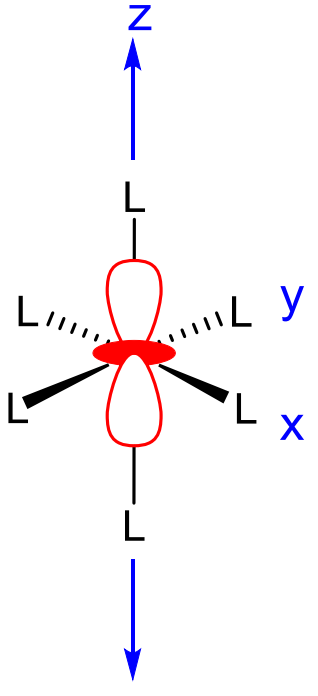
\includegraphics[width=0.5\linewidth]{Imágenes/JTE-z-out-draw.png}
        \caption{}
    \end{subfigure}
    %\hfill % Espacio horizontal entre imágenes
    \begin{subfigure}{0.2\textwidth}
        \centering
        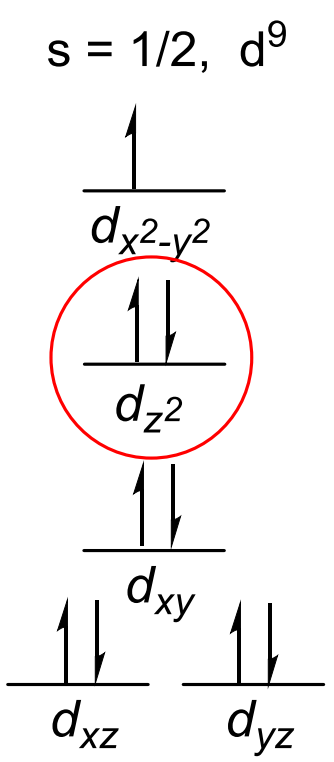
\includegraphics[width=0.5\linewidth]{Imágenes/JTE-z-out-orbitals.png}
        \caption{}
    \end{subfigure}
    
    \vspace{0.5cm} % Espacio vertical entre filas
    
    % Fila inferior: Distorsión z-in (Compresión)
    \begin{subfigure}{0.3\textwidth}
        \centering
        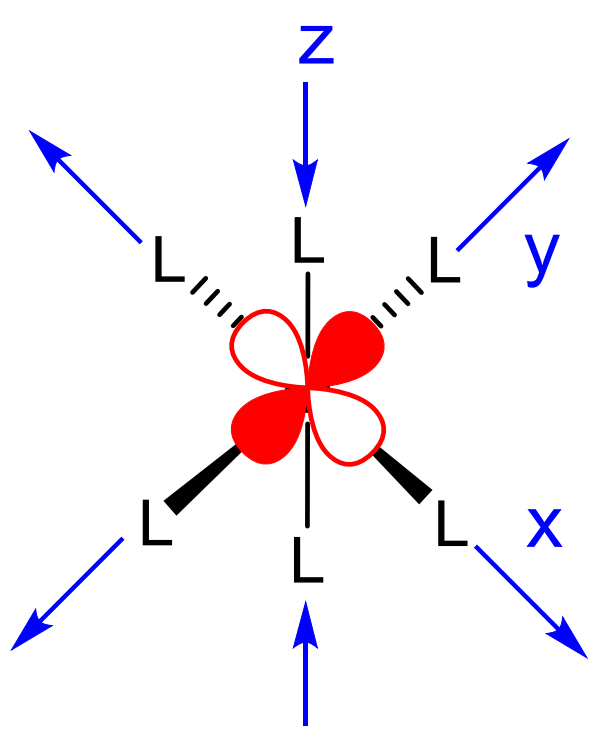
\includegraphics[width=0.5\linewidth]{Imágenes/JTE-z-in-draw.png}
        \caption{}
    \end{subfigure}
    %\hfill % Espacio horizontal entre imágenes
    \begin{subfigure}{0.2\textwidth}
        \centering
        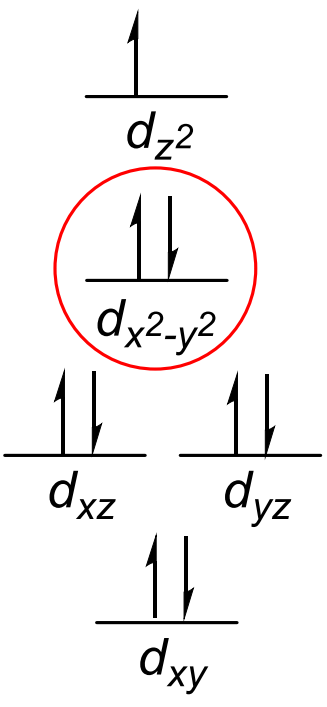
\includegraphics[width=0.5\linewidth]{Imágenes/JTE-z-in-orbitals.png}
        \caption{}
    \end{subfigure}
    
    \caption{Ilustración  del efecto Jahn-Teller de \cite{Cu-2019-01} para un complejo octaédrico del ion Cu(II) con configuración electrónica $d^9$. Arriba se muestra la distorsión por elongación axial (z-out), donde los enlaces axiales se alargan, y su correspondiente desdoblamiento de orbitales. Abajo se presenta la distorsión por compresión axial (z-in), con el acortamiento de los enlaces axiales y su respectivo desdoblamiento energético. La distorsión z-out es la observada más comúnmente en la experimentación .}
    \label{fig:jahn_teller_cu2}
\end{figure}


Aunque la elongación es la geometría más común, estudios teóricos han demostrado que ambas son posibles para el catión \ce{[Cu(OH2)6]^{2+}} \cite{Cu-2019-01}.

El JTE no es un mero detalle, sino la causa directa de la química de coordinación excepcionalmente flexible y dinámica del \ce{Cu^{2+}}. Dota al ion de una plasticidad estructural inusual, permitiéndole adoptar múltiples geometrías (octaédrica distorsionada, piramidal cuadrada, planar cuadrada) con diferencias energéticas muy pequeñas entre ellas. Esta flexibilidad es inherentemente dinámica; en solución, el complejo interconvierte rápidamente entre estas configuraciones. Esto explica la alta labilidad de sus ligandos, cuya tasa de intercambio es órdenes de magnitud superior a la de otros cationes divalentes. La debilidad de los enlaces axiales facilita este rápido intercambio y ha generado un prolongado debate sobre el número de coordinación preferido (4, 5 o 6) del ion en solución.

\section{Hidratación}

\subsection*{Estudios Experimentales}

Históricamente, los estudios experimentales han sido la piedra angular en la comprensión de la solvatación del Cu\textsuperscript{2+}. Las técnicas más utilizadas incluyen:
\begin{itemize}
    \item Difracción de Rayos X y Neutrones
    \item Espectroscopia de Absorción de Rayos X (EXAFS y XANES)
\end{itemize}

Los primeros trabajos de difracción en las décadas de 1970 y 1980 establecieron la idea de una coordinación octaédrica distorsionada (NC=6), con una configuración (4+2) que implicaba cuatro ligandos de agua en posiciones ecuatoriales y dos más distantes en posiciones axiales. Sin embargo, a partir del año 2000, estudios más avanzados, que combinaban técnicas como la difracción de neutrones con dinámica molecular o empleaban análisis de EXAFS y XANES más sofisticados, comenzaron a favorecer un modelo de **coordinación quíntuple (NC=5)** con una geometría de pirámide cuadrada.

Actualmente, existe un consenso experimental sobre las distancias de enlace ecuatoriales ($Cu-O_{eq}$), que se reportan consistentemente en el rango de **1.93--2.00 \AA**. Por el contrario, las distancias axiales ($Cu-O_{ax}$) son más difíciles de medir y presentan una mayor variabilidad, con valores que oscilan entre **2.15 \AA \ y 2.60 \AA**. Investigaciones recientes de alta resolución sugieren incluso la existencia de dos distancias axiales distintas, lo que apunta a un octaedro no centrosimétrico. Algunos estudios que emplean un enfoque multitécnica han llegado a proponer un NC promedio de 4.5, lo que refuerza la idea de una mezcla dinámica de geometrías en solución. La imagen moderna, por tanto, describe una "plasticidad estructural" donde múltiples estados de coordinación coexisten en un equilibrio dinámico.

\subsection*{Estudios Teóricos}

Los estudios computacionales han sido fundamentales para interpretar la evidencia experimental y proporcionar una visión dinámica del proceso de solvatación. Los principales métodos teóricos empleados son:
\begin{itemize}
    \item Teoría del Funcional de la Densidad (DFT)
    \item Dinámica Molecular (MD), tanto clásica como \textit{ab initio} (AIMD)
    \item Métodos híbridos de Mecánica Cuántica/Mecánica Molecular (QM/MM)
\end{itemize}

Las simulaciones teóricas corroboran la naturaleza dinámica del efecto Jahn-Teller, mostrando transformaciones rápidas entre diferentes configuraciones en escalas de tiempo de femtosegundos. Gran parte de los modelos teóricos indican que la geometría de **pirámide cuadrada (NC=5)** es la más estable en solución acuosa, aunque la diferencia de energía con la forma **hexa-coordinada (NC=6)** es muy pequeña ($\sim$1.4 kcal/mol). Esto sugiere que ambas especies pueden coexistir en solución, lo cual está en línea con los hallazgos experimentales más recientes.

Un aporte crucial de los estudios teóricos ha sido resaltar el papel de la segunda capa de solvatación. Se ha demostrado que la formación de enlaces de hidrógeno entre las moléculas de agua de la primera y segunda esfera de hidratación es un factor de estabilización que puede competir energéticamente con la coordinación de una molécula de agua en la posición axial. Las distancias de enlace calculadas concuerdan bien con los datos experimentales, con valores promedio para $Cu-O_{eq}$ de alrededor de **2.00--2.03 \AA** y para $Cu-O_{ax}$ de **2.15--2.30 \AA**. En general, la modelización teórica apoya la visión de un sistema flexible donde coexisten dinámicamente estructuras con NC=5 y NC=6, y descarta una relevancia significativa de la coordinación tetraédrica (NC=4) en el ion Cu\textsuperscript{2+} solvatado en agua.

\section{Solvatación  en Metanol}


Al igual que en el agua, la estructura de solvatación del ion Cu\textsuperscript{2+} en metanol es un área de investigación activa, aunque la cantidad de estudios disponibles es notablemente más escasa. Persiste un debate sobre el número de coordinación (NC) y la geometría predominantes, con diferentes estudios experimentales y teóricos llegando a conclusiones contradictorias. La naturaleza dinámica del ion y la sutil influencia del disolvente complican la obtención de un consenso definitivo. Un resumen detallado de los trabajos más relevantes se encuentra en la Tabla \ref{tab:metanol_corrected}.

\subsection*{Estudios Experimentales}

Las investigaciones experimentales han empleado diversas técnicas espectroscópicas para determinar la estructura local del Cu\textsuperscript{2+} en metanol. Entre los métodos más destacados se encuentran:
\begin{itemize}
    \item Espectroscopia de absorción de rayos X (EXAFS y XANES)
    \item Análisis de modulación de eco de espín de electrones
    \item Estudios de Resonancia Magnética Nuclear (RMN) de Oxígeno-17
\end{itemize}

El panorama experimental se caracteriza por una falta de acuerdo. Mientras que estudios tempranos (Ichikawa y Kevan, 1980) propusieron una coordinación de \textbf{seis (NC=6)}, trabajos posteriores sugirieron que la técnica empleada podría haber sobrestimado las distancias de enlace. Más tarde, estudios de RMN (Helm et al., 1986) observaron una "rápida transición" de isómeros hexacoordinados a conformaciones de \textbf{cinco coordinaciones (NC=5)}, introduciendo la idea de un equilibrio dinámico.

Este debate continúa en estudios más recientes. Por un lado, Zitolo et al. (2012), combinando EXAFS y XANES, concluyeron "inequívocamente" que el Cu\textsuperscript{2+} en metanol adopta una geometría de \textbf{pirámide cuadrada con NC=5}. Por otro lado, un estudio más reciente de Persson et al. (2020) con EXAFS de alta calidad determinó que el mejor modelo de ajuste correspondía a una estructura \textbf{octaédrica distorsionada por Jahn-Teller con NC=6} y carácter no centrosimétrico, contradiciendo directamente la conclusión anterior.

A pesar de la discrepancia en el NC, hay un mayor consenso en las distancias de enlace ecuatoriales ($Cu-O_{eq}$), reportadas consistentemente en el rango de \textbf{1.95--1.98 \AA}. Las distancias axiales ($Cu-O_{ax}$), sin embargo, varían más, con valores reportados de \textbf{2.23 \AA} para el modelo de NC=5 y dos distancias distintas de aproximadamente \textbf{2.20 \AA \ y 2.34 \AA} para el modelo de NC=6.

\subsection*{Estudios Teóricos}

Los métodos computacionales han sido cruciales para explorar el complejo panorama energético de la solvatación del Cu\textsuperscript{2+} en metanol. Las principales técnicas utilizadas incluyen:
\begin{itemize}
    \item Métodos \textit{ab initio} como MP2
    \item Teoría del Funcional de la Densidad (DFT), en particular con el funcional M06-2X
    \item Modelos de disolvente continuo implícito (IEF-PCM)
\end{itemize}

Los estudios teóricos, principalmente los trabajos exhaustivos de Da-yang et al., han demostrado que el NC más estable depende fuertemente de las condiciones del modelo, como el tamaño del clúster de solvente (n), la temperatura y el entorno (fase gaseosa vs. disolvente implícito).

En la \textbf{fase gaseosa}, los cálculos muestran una competencia entre diferentes números de coordinación. El método MP2 tiende a favorecer isómeros \textbf{tetra- y pentacoordinados}, mientras que el método DFT (M06-2X) favorece a los \textbf{penta- y hexacoordinados}. Para clústeres pequeños (n=1-5), las coordinaciones más bajas son las más estables, pero a medida que aumenta el tamaño, las estructuras de mayor NC ganan relevancia.

La inclusión de un \textbf{modelo de disolvente implícito} (IEF-PCM) tiene un "impacto discernible" y cambia drásticamente el panorama. En este entorno, se observa una clara preferencia por los números de coordinación más altos, desfavoreciendo a las estructuras de NC=4. Para clústeres de mayor tamaño (n=7-10), las estructuras \textbf{hexacoordinadas (NC=6)} dominan "exclusivamente" la población a cualquier temperatura. Este hallazgo subraya la importancia crítica del efecto del medio dieléctrico para estabilizar geometrías más compactas y con mayor número de coordinación.

Las distancias de enlace calculadas teóricamente muestran una "excelente concordancia" con los datos experimentales, con valores de $Cu-O_{eq}$ que oscilan entre \textbf{1.94--2.02 \AA} y de $Cu-O_{ax}$ entre \textbf{2.15--2.27 \AA}. Los cálculos también revelan que el disolvente alarga los enlaces dativos axiales en las estructuras pentacoordinadas en comparación con la fase gaseosa.



\section{Justificación y Enfoque Metodológico}

Históricamente, los métodos experimentales como la difracción de rayos X y neutrones o las espectroscopias EXAFS y XANES han sido cruciales para sondear estos sistemas. Sin embargo, a pesar de su capacidad para medir distancias de enlace con precisión, estos métodos enfrentan limitaciones significativas. A menudo existe una considerable controversia y ambigüedad en la determinación del número de coordinación (NC) y la geometría, y resulta técnicamente difícil distinguir entre estructuras con energías muy similares, como las de coordinación cuádruple, quíntuple y séxtuple, que pueden coexistir en solución.

Frente a estas limitaciones, los métodos teóricos y las simulaciones computacionales emergen como una herramienta indispensable y complementaria. Enfoques como la Dinámica Molecular (MD) basada en la Teoría del Funcional de la Densidad (DFT) permiten superar las desventajas experimentales al proporcionar una visión detallada a nivel atómico. Estos métodos posibilitan la exploración de superficies de energía potencial, la caracterización de efectos dinámicos como la inversión del eje de Jahn-Teller en escalas de tiempo de picosegundos, y el estudio de interacciones complejas como la transferencia de carga y los enlaces de hidrógeno, que son difíciles de aislar experimentalmente. Si bien los métodos teóricos no están exentos de desventajas, como el alto costo computacional y una fuerte sensibilidad a la elección del funcional y la base de conjunto, su capacidad para modelar la dinámica y la coexistencia de múltiples estados los convierte en una opción poderosa para resolver las controversias existentes.

El presente trabajo de tesis aprovecha las ventajas de los métodos teóricos para abordar dos frentes. Primero, se enfoca en la solvatación del Cu\textsuperscript{2+} en metanol, un área donde la información experimental y teórica es notablemente más escasa en comparación con el agua. Este vacío de conocimiento representa un área de oportunidad significativa. Por ello, este trabajo presenta por primera vez en la literatura un estudio teórico exhaustivo sobre la estructura y dinámica de los clústeres de Cu\textsuperscript{2+}(MeOH)\textsubscript{n} utilizando DFT. Segundo, se reexamina el caso del agua. Aunque es un sistema mucho más estudiado, la controversia sobre la predominancia de una coordinación quíntuple o séxtuple persiste. El enfoque teórico permite analizar la coexistencia dinámica de estas especies, ofreciendo una perspectiva que las mediciones experimentales, a menudo promediadas en el tiempo, no pueden capturar completamente.

Para llevar a cabo estos estudios, se ha seleccionado el funcional \textbf{M06-2X}. Esta elección se justifica brevemente aquí, y se detallará a profundidad en capítulos posteriores. El M06-2X se presenta como una alternativa computacionalmente eficiente a métodos \textit{ab initio} más costosos como el MP2, y ha demostrado una excelente concordancia con datos experimentales y teóricos para la descripción de los clústeres de Cu\textsuperscript{2+} en metanol, reproduciendo con precisión las distancias de enlace y las reglas de estabilidad.

En los siguientes capítulos se expondrá el marco teórico detallado de la Dinámica Molecular y la Teoría del Funcional de la Densidad, explicando la naturaleza del funcional M06-2X. Posteriormente, se presentará la metodología computacional empleada para la construcción y simulación de los sistemas en ambos disolventes. Finalmente, se realizará un análisis exhaustivo de los resultados y se presentarán las conclusiones derivadas de este estudio computacional.



    % Bibliografía
    \printbibliography

    \backmatter 

\end{document}
